\documentclass{include/protokollclass}
% Main File - Based on protokollclass.cls
% Comments are mostly in English (and some in German, concerning the Praktikum)
% ------------------------------------------------------------------------------
% Further files in folder:
%  - include/cmds.tex (for macros and additional commands)
%  - include/kitlogo.pdf (for titlepage)
%  - lit.bib (bibtex bibliography database)
%  - include/titlepage.tex (for layout of titelpage)
% ------------------------------------------------------------------------------
% Useful Supplied Packages:
% amsmath, amssymb, mathtools, bbm, upgreek, nicefrac,
% siunitx, varioref, booktabs, graphicx, tikz, multicol

\usepackage{rotating}
\usepackage{icomma}
\usepackage{subfig}
\usepackage{pdfpages}
\usepackage[onehalfspacing]{setspace}


%% ---------------------------------------------
%% |    Informationen über dieses Protokoll    |
%% ---------------------------------------------
\newcommand{\praktikum}{P1}                % P1 oder P2
\newcommand{\semester}{WS16/17}            % z.B. "WS14/15" oder "SS15"

\newcommand{\wochentag}{Di}                % Mo, Di, Mi oder Do
\newcommand{\gruppennr}{04}                % Zweistellige Gruppennummer

\newcommand{\nachnamea}{Friedrich}             % Nachname des ersten Praktikanten
\newcommand{\vornamea}{Tabea}               % Vorname des ersten Praktikanten
\newcommand{\nachnameb}{Stockmeier}              % Nachname des zweiten Praktikanten
\newcommand{\vornameb}{Lea}              % Vorname des zweiten Praktikanten

\newcommand{\emailadressen}{lea.stockmeier@web.de, tabea.friedrich@t-online.de}
% optionale Angabe von Emailadresse(n) für den Kontakt mit dem Betreuer

\newcommand{\versuch}{Gesamtübersicht} % Name des Versuchs
\newcommand{\versuchsnr}{80}               % bitte die korrekte Nummer dem 
                                           % Arbeitsplatz am Versuchstag 
                                           % entnehmen
\newcommand{\fehlerrechnung}{Nein}         % Ob Fehlerrechnung im Versuch 
                                           % durchgeführt wurde oder nicht

\newcommand{\betreuer}{M. Mustermann}      % Name des zuständigen Betreuers
\newcommand{\durchgefuehrt}{01.09.16}      % Datum, an dem der Versuch 
                                           % durchgeführt wurde





%% --------------------------------------
%% |    Settings for Word Separation    |
%% --------------------------------------
% Help for separation:
% In German package the following hints are additionally available:
% "- = Additional separation
% "| = Suppress ligation and possible separation (e.g. Schaf"|fell)
% "~ = Hyphenation without separation (e.g. bergauf und "~ab)
% "= = Hyphenation with separation before and after
% "" = Separation without a hyphenation (e.g. und/""oder)

% Describe separation hints here:
\hyphenation
{
    über-nom-me-nen an-ge-ge-be-nen
    %Pro-to-koll-in-stan-zen
    %Ma-na-ge-ment  Netz-werk-ele-men-ten
    %Netz-werk Netz-werk-re-ser-vie-rung
    %Netz-werk-adap-ter Fein-ju-stier-ung
    %Da-ten-strom-spe-zi-fi-ka-tion Pa-ket-rumpf
    %Kon-troll-in-stanz
}





% um die Titelseite per PDF-reader auszufüllen. Vorgefertigte Daten
% können in Datei 'data.tex' modifiziert werden.
%\setboolean{forminput}{true}
% um die Anmerkungen zu den Textfeldern anzeigen zu lassen
%\setboolean{showannotations}{true}
% Erneuern der Seitenzahl in jedem Kapitel
%\setboolean{chapResetPageNumb}{true}
% Einbinden der Kapitelnummer in der Seitenzahl
%\setboolean{chapWiseNumb}{true}
% english or ngerman (new german für neue deutsche Rechtschreibung statt german)
\SelectLanguage{ngerman}

\title{Geophysikalische Geländeübungen \\ SS 2018 \\ Gesamtübersicht}
\subtitle{Messgebiet A59/1 (Riedheim)}
\author{\\ Svenja Müller \\ mueller-svenja@gmx.net
\\ \\und\\ \\
Lea Stockmeier \\ lea.stockmeier@web.de \\ \\ \\
Betreuer: Vorname1 Nachname1 und Vorname2 Nachname2}
\date{\vfill\vfill\vfill \today}


%% -----------------------
%% |    Main Document    |
%% -----------------------
\begin{document}
    % Titlepage und ToC
    \FrontMatter

    \maketitle

    \begingroup \let\clearpage\relax    % in order to avoid listoffigures and
    \tableofcontents                    % listoftables on new pages
    \listoffigures
    \listoftables
    \endgroup
    %\cleardoublepage



    % Contents
    \MainMatter
    
    \emptychapter[1]{Messprotokoll 1}{} % usage: \emptychapter[page displayed 
                                        %        in toc]{name of the chapter}
    \pseudochapter[3]{Messprotokoll 2}  % usage: \pseudochapter[number of pages 
                                        %        added]{name of the chapter}
    
    \chapter{Messstandort}
    %Geammtübersicht Messgebiet

\section{Das Hegau}
Das Hegau ist eine Gebiet dass grob zwischen dem Bodensee und der schwäbischen Alb liegt(Wikipedia)???. Charakteristisch für dieses Gebiet sind die vulkanisch 
geprägten Hegauer Kegelberge. Diese Kegelberge sind Schlothe erlöschener Vulkane. Der Vulkanismus des Hegaugebiets hat seinen Ursprung in der Mitte des Miozän, 
was vor etwa 14 Millionen Jahren war. Es entstanden duzende Vulkane, in deren Schlothe vor ca. 9 Millionen Jahren auch der Hegauer Basalt erstarrte.\\
Im Pleistozän gab es eine Eiszeit in diesem Gebiet. Durch die entstandenen Kletscher wurde Molasse und Tuff abgetragen, es blieben, die heute noch zu sehenden, 
Phonolithkerne und Basaltkerne stehen. 



\newpage


\section{Die Messgebiete}


Es gab im Wesentlichen zwei Messgebiete auf denen wir unsere Messungen durchgeführt haben, sie liegen über Riedheim. In Abbildung \ref{abb:Messgebiete} sind diese Messgebiete 
eingezeichnet. Unter Messgebiet 1 liegt der Basaltgang, hier wurde mit allen vier Messmethoden Messungen durchgeführt. 
Auf Messgebiet 2 wurde nur mit Geoelektrik und Seismik gemessen.
gemessen.
\begin{figure}[h]
 \centering
<<<<<<< HEAD
 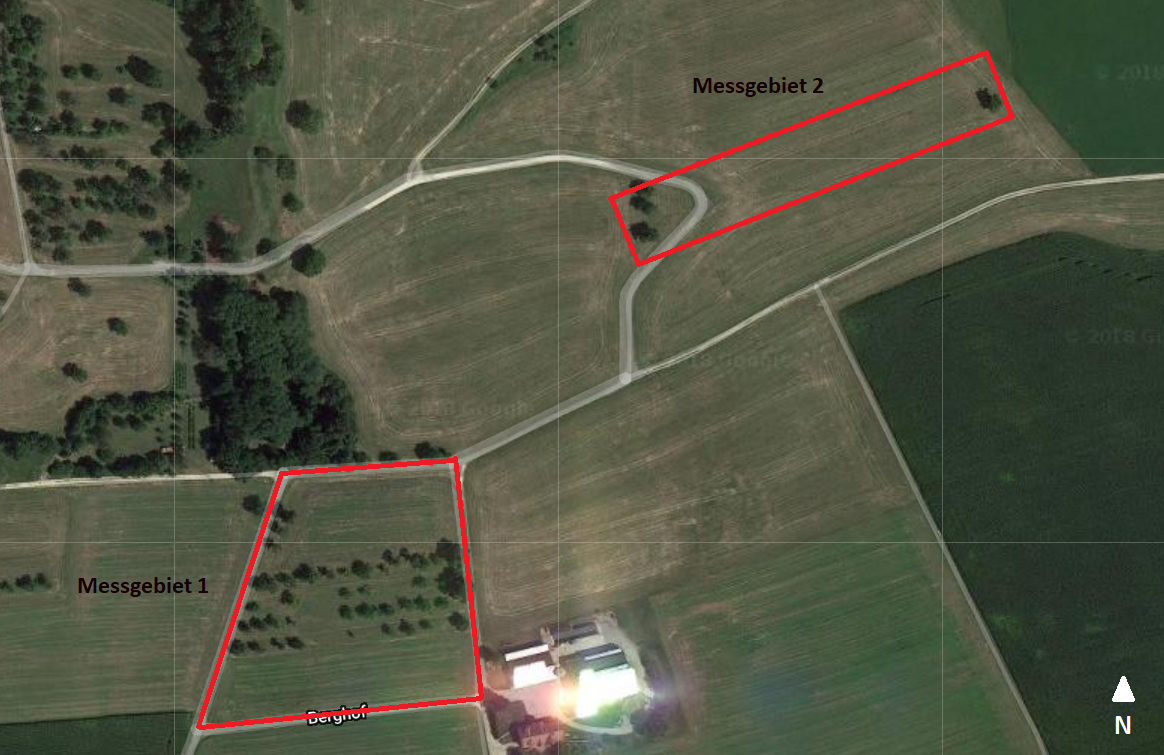
\includegraphics[width=0.9\textwidth]{fig/Messgebiete.pdf}
 \caption[Messgebiete]{Messgebiete auf denen unsere Messungen durchgeführt wurden. Unter Messgebiet 1 ist der Basaltgang.}
=======
 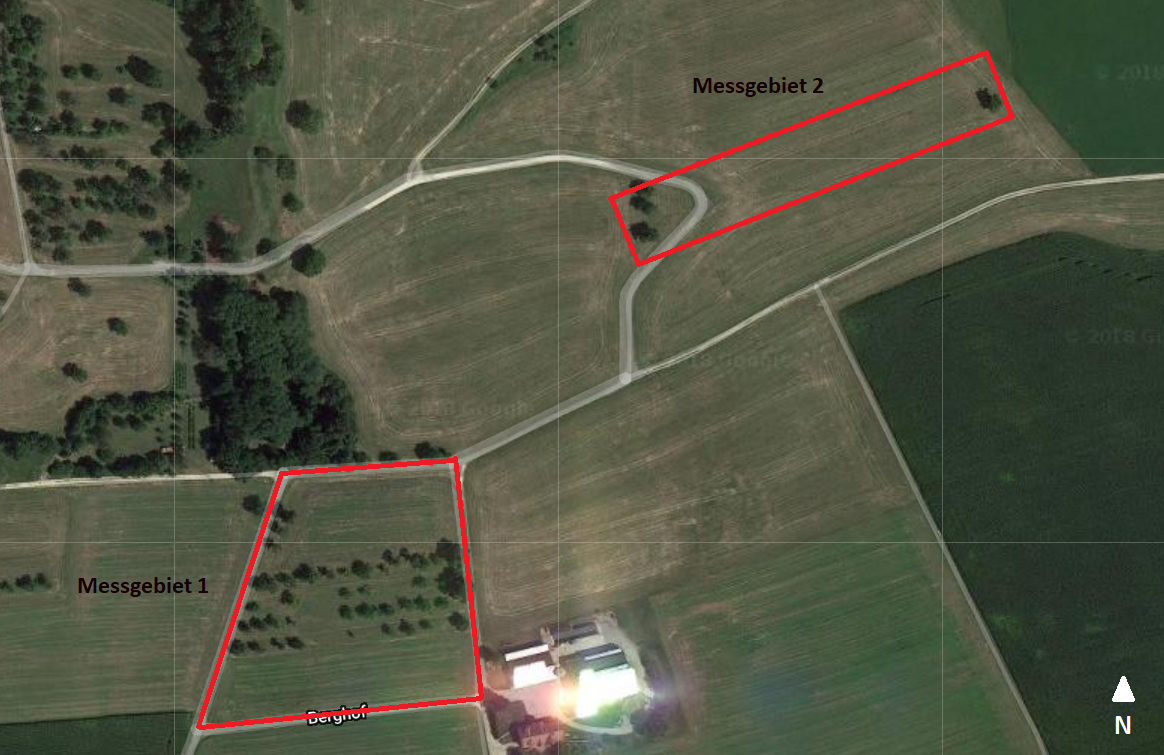
\includegraphics[width=0.9\textwidth]{fig/Messgebiete.png}
 \caption[Messgebiete]{Messgebiete auf denen unsere Messungen durchgeführt wurden. Unter Messgebiet 1 ist der Basaltgang. Die Graphik wurde von Rebekka Kirchgässner und Luisa Rank übernommen.}
>>>>>>> d0ea8881a3c938a2c47a0a3fbea97a2dc90b3a2a
 \label{abb:Messgebiete}
\end{figure}

Aberhalb den Messgebiets 1 ist eine Steinbruch in dem Basalt frei gelegt ist. Der Aufschluss dieses Basaltgangs ist etwa 5 Meter hoch und 16 Meter breit. 
Es ist zu erkennen, dass der Basalt nicht im ganzen Aufschuss in gleichem Zustand vorliegt. In der Mitte sieht er wesentlich kompakter aus als an den Rändern.
Dieser Basaltgang geht unterirdisch weiter und läuft schräg durch das Messgebiet 1. Bei den meisten unserer Messungen wurde der Basaltgang untersucht.

\begin{figure}[h]
 \centering
 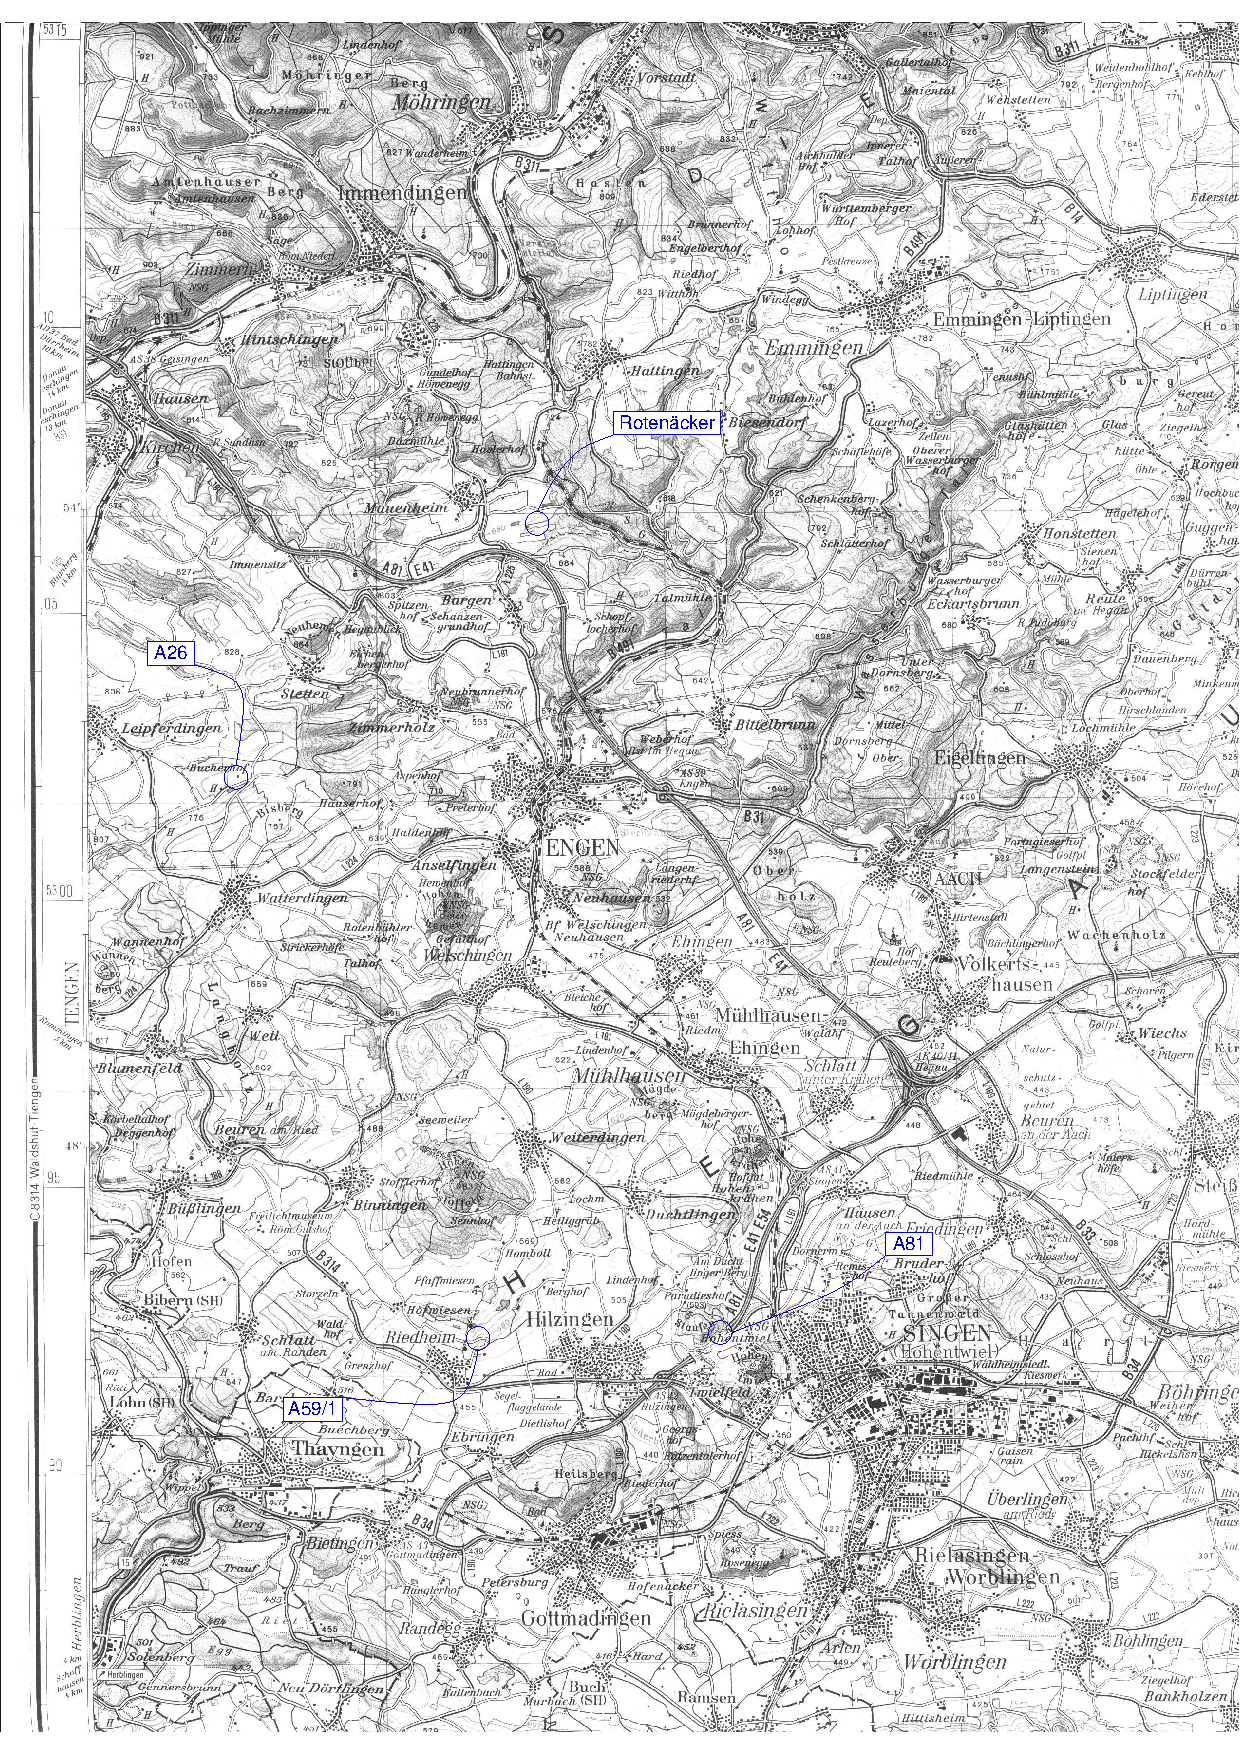
\includegraphics[width=0.9\textwidth]{fig/Uebersichtskarte der Messgebiete.pdf}
 \caption[Messgebiete]{Messstandorte auf denen die Geländeübung durchgeführt wurde. Unser Messstandort Riedheim ist unten links (A59/1) eingezeichnet.}
 \label{abb:Messgebiete}
\end{figure}
<<<<<<< HEAD
=======

In Abbildung \ref{abb:Geolog} ist eine Geologische Karte unseres Messgebiets zu sehen. In der Mitte ist in schwarz der Basaltgang oberhalb des Steinbruchs zu sehen, denn dort wurde er sicher nachgewiesen.
Unterhalb des Steinbruchs ist die Lage des Basaltgangs durch zwei gestrichelte Linien angegeben, da hier nicht eindeutig nachgewiesen wurde ob es sich um Basalt handelt. Der Untergrund unter dem Messgebiet 1 besteht nach dieser Karte aus älterem Juranagelfluh. Dies wurde der Legende der Karte entnommen. Das Messgebiet 2 liegt teilweise über älterem Juranagelfluh und oberer Süßwassermolasse.

\begin{figure}
 \centering
 \includegraphics[width=0.9\textwidth]{fig/Geolog.pdf}
 \caption[Geologische Karte]{Geologische Karte des Messstandorts Riedheim}
 \label{abb:Geolog}
\end{figure}


>>>>>>> d0ea8881a3c938a2c47a0a3fbea97a2dc90b3a2a
 %\cleardoublepage
    
     \chapter{Fragestellung}
    %Gesammtübersicht Fragestellung
Während der Messwoche der geophysikalischen Geländeübungen wurden vier verschiedenen Messmethoden verwendet, die Refraktionsseismik, Geoelektrik, Gravimetrie und Magnetik. An erster Stelle stand bei
uns die Fragestellung in wieweit sich die Ergebnisse dieser Messmethoden unterscheiden. Dadurch wollten wir die Messverfahren besser verstehen und einschätzen können welchen Einfluss die Wahl des Messverfahrens auf die Ergebnisse hat.

Wie bereits im Abschnitt Messgebiet beschrieben, wird unter Messgebiet 1 ein Basaltgang vermutet. Unser zweites Ziel war es, dessen Lage möglicht genau zu bestimmen. 


Wir wussten zwar, dass der Basaltgang eigentlich nicht mit der Seismik vermessen werden kann,
wollten dies aber Überprüfen und herausfinden in wiefern unsere Messergebnisse durch den Basaltgang beeinflusst worden sein könnten. Das Profil auf dem die Messung durchgeführt wurde ist in 
Abbildung \ref{abb:Seismik} als S21-S22 zu sehen.
Die Seismikmessung auf Messgebiet 2 wurde durchgeführt, um ein Verfahren zu haben mit dem die geoelektrikmessung verglichen werden kann und um gute Ergebnisse für die Auswertung zu haben.
Das Profil S31-S32 auf Messgebiet 2 war relativ lang und eben,wie man in Abbildung \ref{abb:Seismik} erkennt, so das wir davon ausgingen hier gut eine Schichtgrenze finden zu können.

\begin{figure}
 \centering
 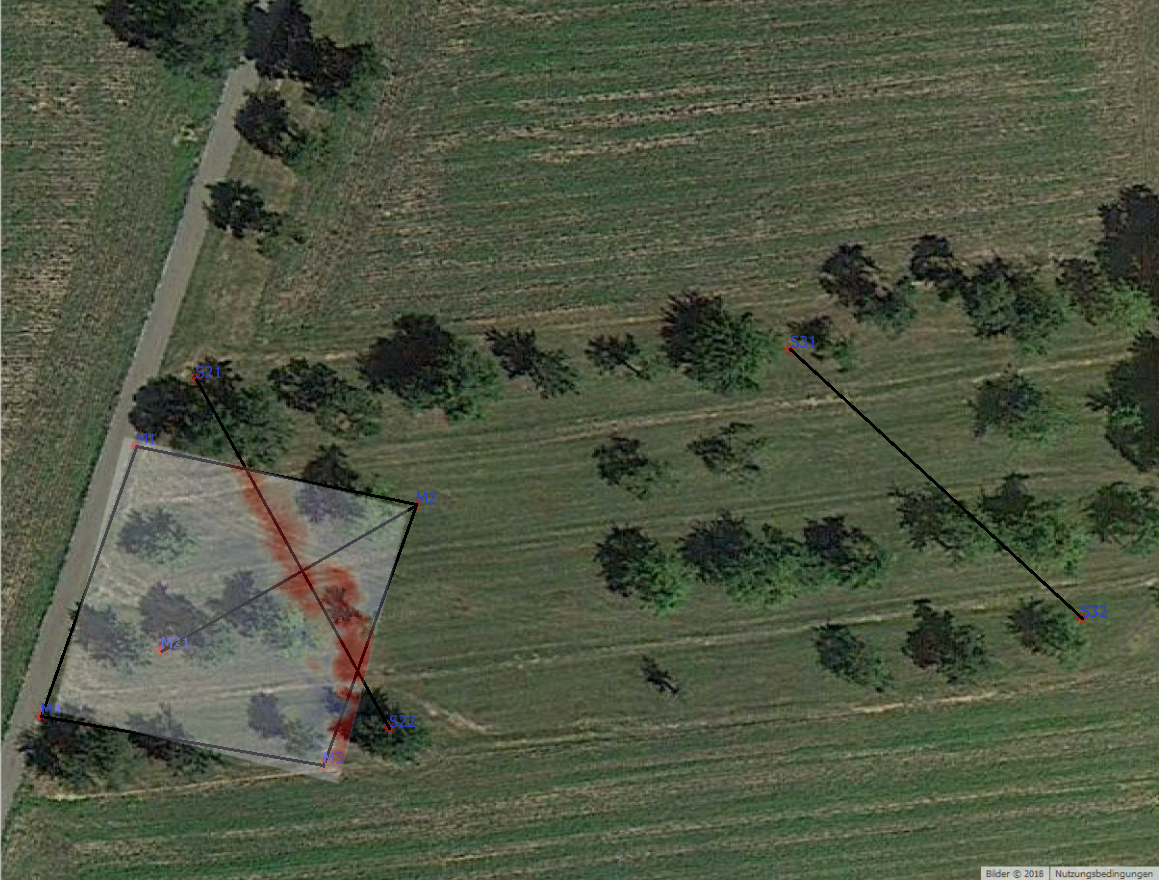
\includegraphics[width=0.9\textwidth]{fig/Seismik.png}
 \caption[Die Seismik- Messprofile S11-S21, S21-S22]{Die Seismik- Messprofile S11-S21, S21-S22. Die Graphik wurde von Rebekka Kirchgässner und Luisa Rank übernommen.}
 \label{abb:Seismik}
\end{figure}

Die Magnetig wurde am ersten Tag durchgeführt. Hier war es uns bei der Kartierung wichtig zunächst die Lage des Basaltgangs festzustellen, um alle weiteren Messungen durchführen zu können.
Das Gebiet, auf dem die Kartierung zu sehen ist, ist in Abbildung \ref{abb:Kart} abgebildet. Die restlichen Messungen wurden auf den Profilen, die in Abbildung \ref{abb:Magnetig} eingezeichnet durchgeführt.
Hier war unsere Fragestellung wieder wie gut sich die Magnetik im Vergleich zu den anderen Messverfahren zu lokalisieren des Basaltgangs eignet.

\begin{figure}
 \centering
 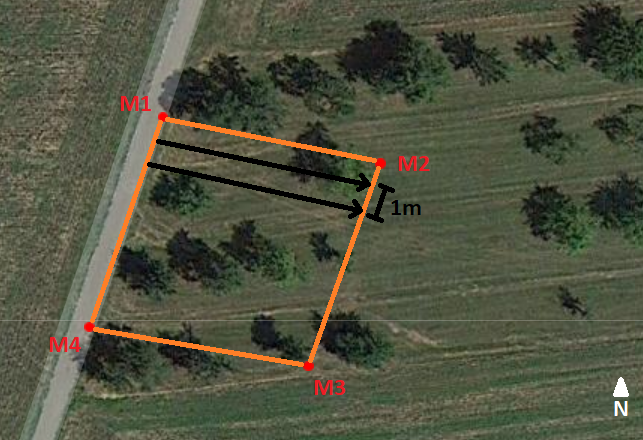
\includegraphics[width=0.9\textwidth]{fig/Kartierunggps.png}
 \caption[{Lage der Magnetk-Kartierung]{Lage der Magnetk-Kartierung. Die Graphik wurde von Rebekka Kirchgässner und Luisa Rank übernommen.}
 \label{abb:Kart}
\end{figure}

\begin{figure}
 \centering
 \includegraphics[width=0.9\textwidth]{fig/MagnetikGesammtueberblick.png}
 \caption[Gesammtübersicht über die Profile der Magnetig]{Gesammtübersicht über die Profile der Magnetig. Die Graphik wurde von Rebekka Kirchgässner und Luisa Rank übernommen.}
 \label{abb:Magnetik}
\end{figure}

Bei der Geoelektrik wurde wieder auf beiden Messgebieten eine Messung durchgeführt. Die Sondierung wurde auf einem Profil über dem der Seismik am Messgebiet 2 durchgeführt, dies ist in 
Abbildung ... eingezeichnet. Die Messung wurde durchgeführt um zu sehen ob wir Schichtgrenzen finden, und wenn ja ob diese mit denen der Seismik übereinstimmen.
Die Tomographie und Wenner-kartierung, Profil E11-E12, wurde wie schon Messungen der Magnetik und Gravimetrie orthogonal zum Basaltgang durchgeführt, um die Messergebnisse dieser drei Verfahren
miteinander vergleichen zu können. Die beiden Profile sind in Abbildung \ref{abb:Geoelek} abgebildet.

\begin{figure}
 \centering
 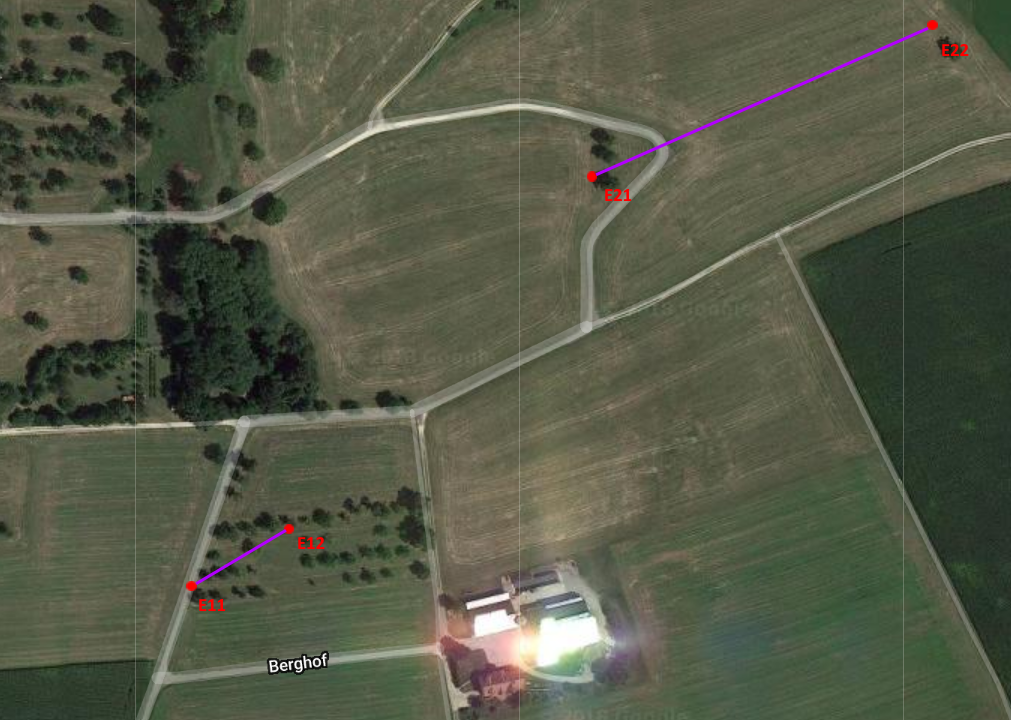
\includegraphics[width=0.9\textwidth]{fig/profilegps.png}
 \caption[Profile der Geoelktrik]{Profile der Geoelektrik. Die Graphik wurde von Rebekka Kirchgässner und Luisa Rank übernommen. }
 \label{abb:Geoelek}
\end{figure}

Da die Gravimetrie-Messung sehr viel Zeit in gebraucht hat, wurde nur eine Messung, auf Profil G11-G12, zu sehen in Abbildung \ref{abb:Geoelek2}, durchgeführt. Wir haben gehofft genau genug
messen zu können um den Basaltgang zu sehen und eventuell ähnliche Ergebnisse wie die bereits beschriebenen Messmethoden zu haben.

\begin{figure}
 \centering
 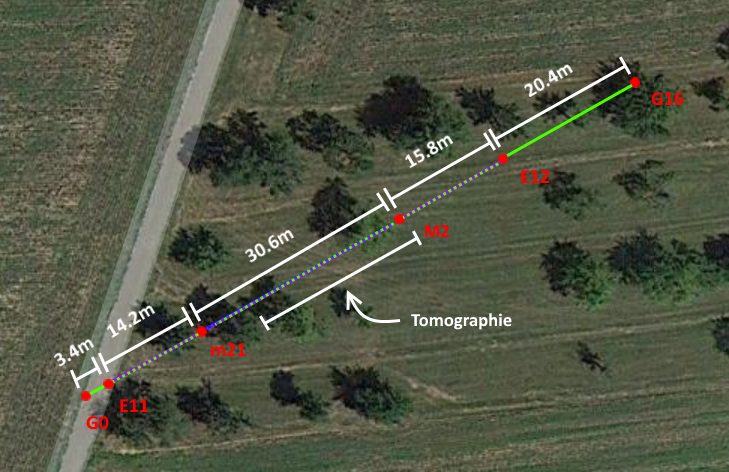
\includegraphics[width=0.9\textwidth]{fig/ElektrikMagnetikGravimetrie0gps.png}
 \caption[Profil der Gravimetrie]{Profil der Gravimetrie. Die Graphik wurde von Rebekka Kirchgässner und Luisa Rank übernommen. }
 \label{abb:Geoelek2}
\end{figure}






 %\cleardoublepage

    % appendix for more or less interesting calculations
    \Appendix
    \chapter*{\appendixname} \addcontentsline{toc}{chapter}{\appendixname}
    % to make the appendix appear in ToC without number. \appendixname = 
    % Appendix or Anhang (depending on chosen language)
    \section{Messprotokolle}

\begin{figure}[h!]
 \centering
 \includegraphics[width=0.8\textwidth]{fig/Messprotokolle/Kalibrierung.png}
 \caption{Messprotokoll zur Kalibrierungsmessung}
 \label{fig:MPKalibrierung}
\end{figure}

\begin{figure}[h!]
 \centering
 \includegraphics[width=\textwidth]{fig/Messprotokolle/EinflussHuette.png}
 \caption{Messprotokoll zum Profil zur Untersuchung der Einflüsse äußerer Störfaktoren auf die Basismessung}
 \label{fig:MPHuette}
\end{figure}

% \begin{figure}[h!]
%  \centering
%  \includegraphics[width=\textwidth]{fig/Messprotokolle/}
%  \caption{}
%  \label{fig:}
% \end{figure} %\cleardoublepage



    % Bibliography
    \TheBibliography

    % BIBTEX
    % use if you want citations to appear even if they are not referenced to: 
    % \nocite{*} or maybe \nocite{Kon64,And59} for specific entries
    %\nocite{*}
    \bibliographystyle{babalpha}
    \bibliography{lit.bib}

    % THEBIBLIOGRAPHY
    %\begin{thebibliography}{000}
    %    \bibitem{ident}Entry into Bibliography.
    %\end{thebibliography}
\end{document}
